\documentclass[11pt,a4paper]{article}
\usepackage[T1]{fontenc}
\usepackage[latin1]{inputenc}
\usepackage{lmodern}
\usepackage{a4wide}
\usepackage[dvips]{graphicx}

\usepackage{float}

\usepackage[
pdfauthor={ACE Project Team},
pdftitle={User Manual},
pdfcreator={pdftex},
]{hyperref}

\usepackage{sectsty}
\allsectionsfont{\sffamily}

\usepackage{fancyheadings} 
\pagestyle{fancy} 
\lhead{\textsf{\textbf{ACE} \\ \small{a collaborative editor}}}
\chead{}
\rhead{
\parbox[c]{3cm}{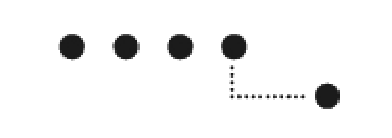
\includegraphics[height=0.875cm,width=3cm]{../../images/logo_BFH.eps}}
\parbox[c]{2.2cm}
{\tiny{\textsf{Berner Fachhochschule \\
Hochschule f�r \\
Technik und Informatik}}}}
\lfoot{}
\cfoot{\textsf{\thepage}}
\rfoot{}
\setlength{\headrulewidth}{0.6pt}
\setlength{\footrulewidth}{0.6pt}
\setlength{\topmargin}{-50pt}
\addtolength{\headheight}{50pt}

\usepackage{colortbl}

\newcommand{\headercol}[2]{\multicolumn{1}{|>{\bfseries\columncolor[gray]{0.82}}p{#1}|}{\textsf{#2}}}
\newcommand{\ace}[0]{\emph{ACE }}



\begin{document}

\setlength{\parindent}{0pt}

\begin{titlepage}
\thispagestyle{empty}
  
\includegraphics[height=1.5in]{../images/pix.eps}

  \begin{center}

    {\fontsize{40}{45} \textbf{\textsf{ACE}}} \\
    \textsf{a collaborative editor} \\
        
    \vspace{36pt}
        
    {\huge{\textbf{\textsf{}}}} \\

    \vspace{36pt}

	\textsf{Berne University of Applied Sciences} \\
    \textsf{School of Engineering and Information Technology} \\
    
  \end{center}

  \vfill
  
  \begin{tabular}{ll}
   \hline

   \\

   \multicolumn{1}{>{\bfseries}p{1.5in}}{\textsf{Date:}} &
   \multicolumn{1}{>{}p{4.3in}}{\textsf{08.11.2005}}          \\
   
   \\
   
   \multicolumn{1}{>{\bfseries}p{1.5in}}{\textsf{Version:}}     &   
   \multicolumn{1}{>{}p{4.3in}}{\textsf{0.1}}                 \\

   \\
   
   \multicolumn{1}{>{\bfseries}p{1.5in}}{\textsf{Projectteam:}}                 &
   \multicolumn{1}{>{}p{4.3in}}{\textsf{Mark Bigler (biglm2@hta-bi.bfh.ch)}}  \\
   \multicolumn{1}{>{\bfseries}p{1.5in}}{}                                      &
   \multicolumn{1}{>{}p{4.3in}}{\textsf{Simon Raess (rasss@hta-bi.bfh.ch)}}    \\
   \multicolumn{1}{>{\bfseries}p{1.5in}}{}                                      &
   \multicolumn{1}{>{}p{4.3in}}{\textsf{Lukas Zbinden (zbinl@hta-bi.bfh.ch)}} \\   
   
   \\
   
   \multicolumn{1}{>{\bfseries}p{1.5in}}{\textsf{Receivers:}}                       &
   \multicolumn{1}{>{}p{4.3in}}{\textsf{Jean-Paul Dubois (doj@hta-bi.bfh.ch)}}       \\
   \multicolumn{1}{>{\bfseries}p{1.5in}}{}                                          &
   \multicolumn{1}{>{}p{4.3in}}{\textsf{Claude Fuhrer (frc@hta-bi.bfh.ch)}}       \\

   \\
   
   \multicolumn{1}{>{\bfseries}p{1.5in}}{\textsf{Location:}}               &   
   \multicolumn{1}{>{}p{4.3in}}{\textsf{Subversion Repository}} \\

   \\  
   
   \hline
  \end{tabular}

\end{titlepage}


\tableofcontents






\newpage
% 1. INTRO
\section{Introduction}

The \textit{User Manual} contains information about how to install and use the application ACE. 






% 2. INSTALLATION
\section{Installation}
To run ACE, you need the following software installed on your computer:
\begin{itemize}
 \item Java Runtime Environment (JRE) - 1.4.2 or higher \\
 Download: \href{http://java.sun.com/j2se/1.5.0/download.jsp}{http://java.sun.com/j2se/1.5.0/download.jsp}
 \item Bonjour (Only for Windows) \\
 Download: \href{http://www.apple.com/downloads/macosx/apple/bonjourforwindows.html}{http://www.apple.com/downloads/macosx/apple/bonjourforwindows.html}
\end{itemize}

Downloads for Linux and other Operating Systems:

\begin{itemize}
 \item Bonjour \\
 Download: \href{http://developer.apple.com/networking/bonjour/download}{http://developer.apple.com/networking/bonjour/download}
 \item Apache Ant \\
 Download: \href{http://ant.apache.org/}{http://ant.apache.org/}
 \item Maven Ant Task \\
 Download: \href{http://maven.apache.org/}{http://maven.apache.org/}
\end{itemize}

% 2.1 MAC
\subsection{Macintosh}
Mac OS X users do not have to install any other software beside ACE itself. The current version of ACE can be downloaded from \href{http://ace.iserver.ch}{http://ace.iserver.ch}.

% 2.2 LINUX
\subsection{Linux and other Operation Systems}
Chances are high that if there is a Java Runtime Environment for your operating system, ACE will work. Unfortunately, there is no installer for Bonjour on Posix operating systems. That means, you have to build Bonjour from source. In the following instructions, replace \texttt{os=linux} with your operating system. Check the Makefile in \texttt{mDNSPosix/Makefile} for supported operating systems.


\begin{enumerate}
\item download the source code
\item unpack the downloaded tar.gz to a location of your choice
\item go to the subdirectory \texttt{mDNSPosix}
\item in the Makefile, adjust the variable \textit{JDK} to point to the correct JDK location
\item type make \texttt{os=linux} to build the \texttt{mDNSResponder}
\item as root user, type \texttt{make os=linux install} to install the \texttt{mDNSResponder} daemon
\item now, the daemon needs to be started by running the startup script \texttt{/etc/init.d/mdns start} as root
\end{enumerate}

Further, you have to build a shared library in order that Bonjour for Java works:

\begin{itemize}
\item in the directory \texttt{mDNSPosix} type \texttt{make os=linux Java}
\item as root, copy the file \texttt{libjdns\_sd.so} from \texttt{build/prod} to somewhere into the Java library path (system property java.library.path)
\end{itemize}

Next you can download the current version of ACE for other platforms from \href{http://ace.iserver.ch}{http://ace.iserver.ch}. To run ACE, type \texttt{ant run} in the top-level directory. Note: you need Apache Ant and Maven Ant Task installed in that case.

% 2.3 WINDOWS
\subsection{Windows}
Windows users have to install a Java Runtime Environment (JRE) - 1.4.2 or higher. Further, Bonjour for Windows has to be downloaded and installed. The ACE installer guides your through the installation and warns you, if Bonjour is not installed. \\
 \\
The current version of ACE can be downloaded from \href{http://ace.iserver.ch}{http://ace.iserver.ch}.





\newpage
% 3. OVERVIEW
\section{Overview}
This section gives you an overview of the ACE Graphical User Interface (GUI). 

\begin{figure}[H]
\begin{center}
  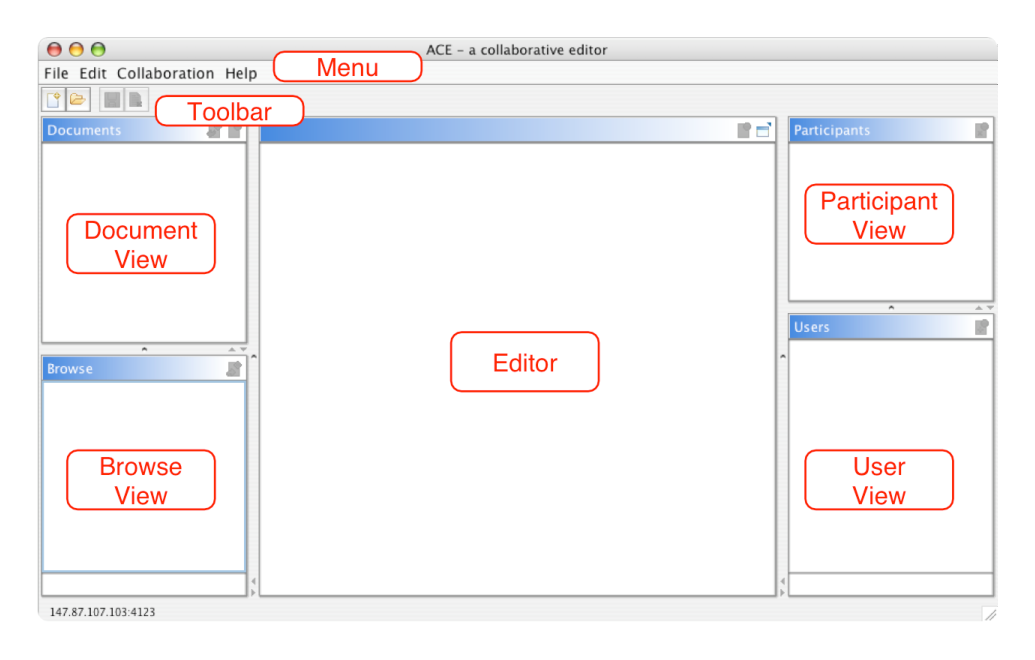
\includegraphics[height=3.135in, width=5.01in]{../images/usermanual/g_ace_overview.eps}
\caption{ACE Overview}
\label{ace_overview}
\end{center}
\end{figure}

% 3.1 MENUS
\subsection{Menu}
The menus (see figure \ref{ace_overview}) are needed to operate the editor. Each menu entry contains multiple actions.
\begin{itemize}
\item File Menu: This menu contains the basic editor functions like create new, open and save documents. Further it provides access to the preferences and has an item to quit the application. See section \ref{first_steps} for a more detailed description of those functions.
\item Edit Menu: This menu contains edit-related actions like cut, copy, paste \& select all.
\item Collaboration Menu: This menu contains actions related to the collaboration functionality described in section \ref{sect_networking}.
\item Help Menu: This menu contains some additional entries. For example you can open the about box which gives you information about the version of ACE you are using.
\end{itemize}

% 3.2 TOOLBAR
\subsection{Toolbar}
The toolbar (see figure \ref{ace_overview}) contains the most used actions.
\begin{figure}[H]
\begin{center}
  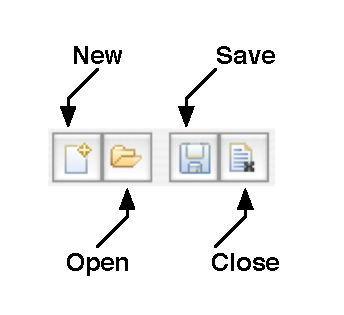
\includegraphics[height=2.26in, width=2.46in]{../images/usermanual/g_toolbar_new2.eps}
\caption{ACE Toolbar}
\label{ace_toolbar}
\end{center}
\end{figure}

% 3.3 EDITOR
\subsection{Editor}
The editor (see figure \ref{ace_overview}) is the main component of ACE. It displays the text of your documents. There is a simple but very useful feature to gain more writing space. Press the button (marked red in the figures below) or double click with your mouse on the editor title (top bar of the editor) to toggle between normal and full screen editing mode.

\begin{figure}[H]
\begin{center}
  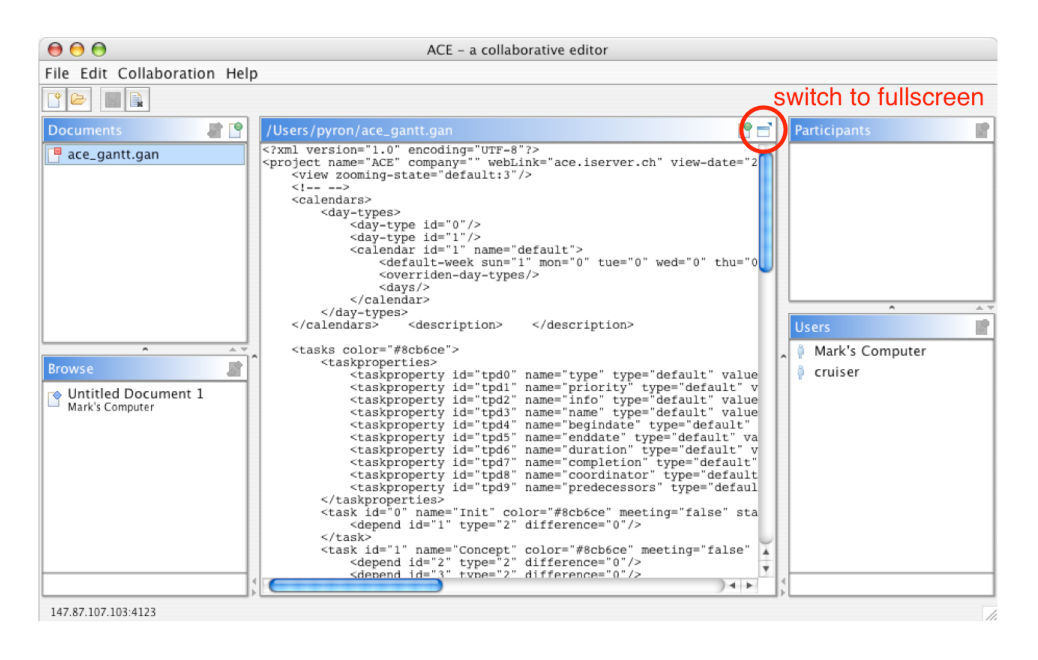
\includegraphics[height=2.09in, width=3.34in]{../images/usermanual/g_editor_normalscreen.eps}
\caption{ACE in normal editing view}
\label{ace_editor_normal}
\end{center}
\end{figure}

\begin{figure}[H]
\begin{center}
  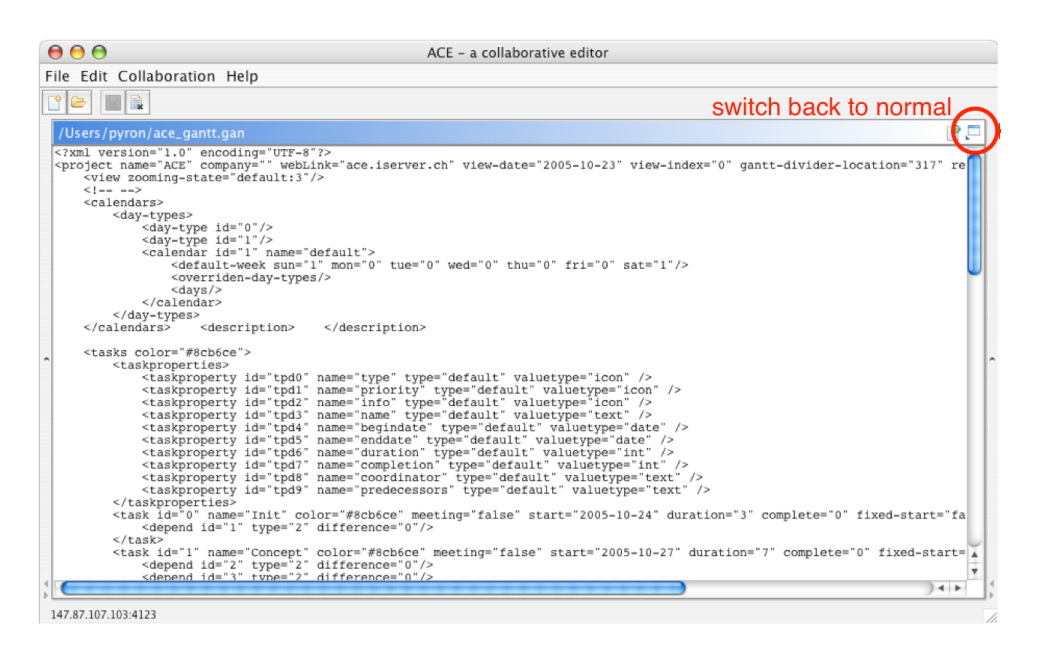
\includegraphics[height= 2.09in, width=3.34in]{../images/usermanual/g_editor_fullscreen.eps}
\caption{ACE in fullscreen editing view}
\label{ace_editor_full}
\end{center}
\end{figure}

% 3.4 VIEWS
\subsection{Views}
ACE has four views, which are arranged around the editor. The \textit{Document View} helps you to manage your open documents. The \textit{User View} displays all other users running ACE in your network. The \textit{Browse View} shows their documents and if you are writing with other users in the same document you see all the participants of the current session in the \textit{Participant View}.

Moreover each view has a toolbar which is placed at the right side in the border at the top. This toolbar contains the most used actions corresponding to the view.


% 3.4.1 DOCUMENT VIEW
\subsubsection{Document View}
The \textit{Document View} shows all your currently open documents. Basically there are three different document types. \textit{Local documents} are documents on your local machine. ACE provides the standard actions to manage the local documents such as \textit{create new}, \textit{open}, \textit{save} and \textit{close} documents. Further, you can publish (see \ref{publish_conceal_documents}) your local documents to make them accessible to other users (\emph{published documents}). \textit{Joined documents} are documents published by other users which you have joined. See section \ref{join_leave_documents} for more informations about joining documents.

\begin{figure}[H]
 \centering
 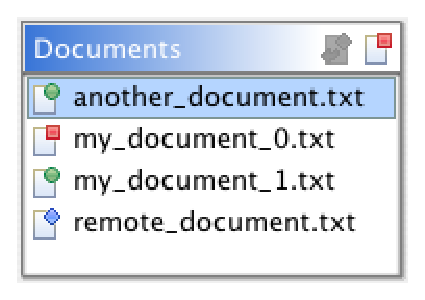
\includegraphics[height=1.78in, width=2.61in]{../images/usermanual/dview_overview.eps}
\caption{Document View}
\label{view_document}
\end{figure}

Different images for each document type makes them well distinguishable (from left to right, icon for the document types: local, published \& remote):

\begin{figure}[H]
\begin{center}
  
\includegraphics[height=32pt, width=32pt]{../images/usermanual/icon_local.eps}
\hspace{10pt}
  
\includegraphics[height=32pt, width=32pt]{../images/usermanual/icon_published.eps}
\hspace{10pt}
  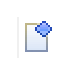
\includegraphics[height=32pt, width=32pt]{../images/usermanual/icon_remote.eps}
\caption{Document Icons}
\label{document_icons}
\end{center}
\end{figure}

% 3.4.2 USER VIEW
\subsubsection{User View}
The \textit{User View} shows all other users currently using ACE on your local area network (LAN). The view has an action to invite other users to your published documents (see section \ref{invite_kick_users}).

\begin{figure}[H]
\begin{center}
  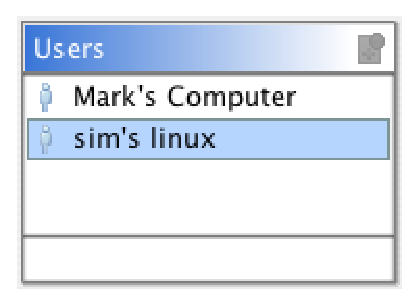
\includegraphics[height=1.82in, width=2.57in]{../images/usermanual/uview_overview.eps}
\caption{User View}
\label{view_user}
\end{center}
\end{figure}

To avoid a crowded list with usernames you can use the \textit{User View} filter. Typing a full username or just parts of it into the textfield below excludes all users that do not match the filter.

\begin{figure}[H]
\begin{center}
  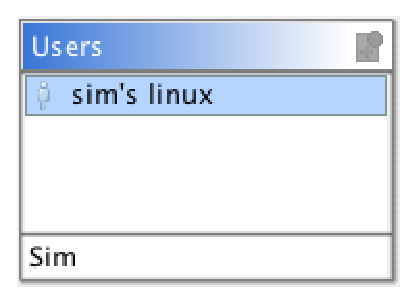
\includegraphics[height=1.81in, width=2.56in]{../images/usermanual/uview_filtering.eps}
\caption{User View Filtering}
\label{view_user_filter}
\end{center}
\end{figure}

% 3.4.3 BROWSE VIEW
\subsubsection{Browse View}
The \textit{Browse View} contains a list with all published documents that can be found on the local area network. Each list entry contains the document title and the name of the publisher. You need this list to join published documents (see section \ref{join_leave_documents}).

\begin{figure}[H]
\begin{center}
  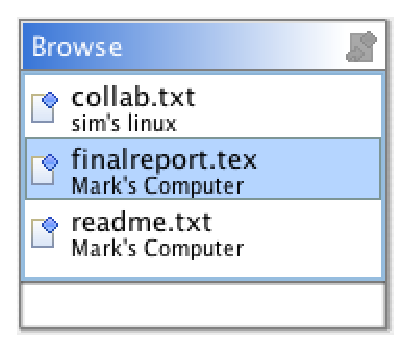
\includegraphics[height=2.12in, width=2.51in]{../images/usermanual/bview_overview.eps}
\caption{Browse View}
\label{view_browse}
\end{center}
\end{figure}

The filtering function helps you to find documents from a specified user. Simply type fragments of the username your are looking for into the text field at the bottom of the view.

\begin{figure}[H]
\begin{center}
  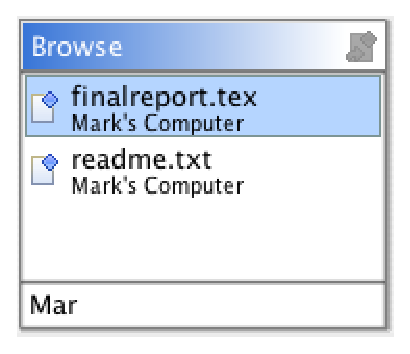
\includegraphics[height=2.14in, width=2.51in]{../images/usermanual/bview_filtering.eps}
\caption{Browse View Filtering}
\label{view_browse_filter}
\end{center}
\end{figure}

% 3.4.4 PARTICIPANT VIEW
\subsubsection{Participant View}
When you publish or join a network document you can see a list of all participants in the \textit{Participant View}. Each participant has his own color which is showed on the right side of his username. These colors are used to highlight the text and to draw the cursor or selection of the corresponding participant. If you are the owner of the document you can select a participant and kick him from the current document (see section \ref{invite_kick_users}).

\begin{figure}[H]
\begin{center}
  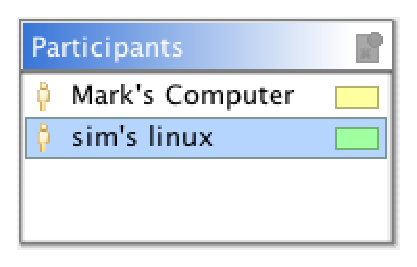
\includegraphics[height=1.56in, width=2.56in]{../images/usermanual/pview_overview.eps}
\caption{Participant View}
\label{view_participant}
\end{center}
\end{figure}


% 3.6 PREFERENCES
\subsection{Preferences}
The preference dialog can be found in the file menu (menu name \textit{Settings}). You need it to change your current settings like user name, the font size or the default encoding. The encoding is only used to load and save documents. The default encoding is ISO-8859-1.

\begin{figure}[H]
\begin{center}
  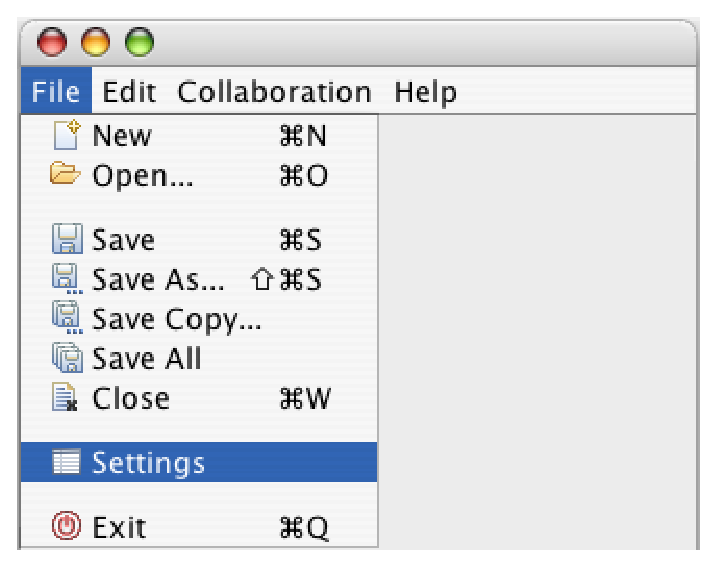
\includegraphics[height=1.78in, width=2.28in]{../images/usermanual/menu_file_preferences.eps}
\caption{Preferences Menu}
\label{view_preferences_menu}
\end{center}
\end{figure}

\begin{figure}[H]
\begin{center}
  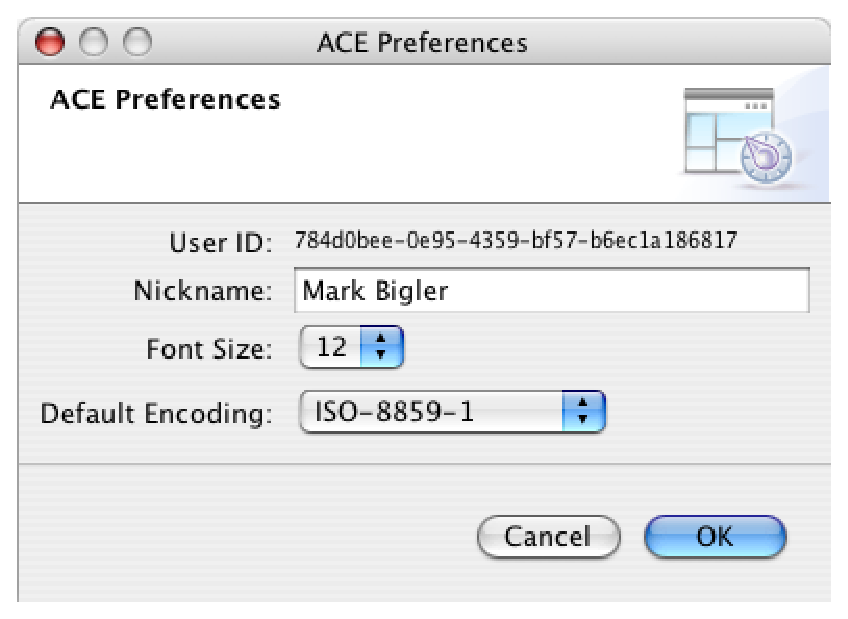
\includegraphics[height=1.95in, width=2.71in]{../images/usermanual/ace_preferences.eps}
\caption{Preferences Dialog}
\label{view_preferences_dialog}
\end{center}
\end{figure}

% 3.7 ABOUT
\subsection{About}
The about dialog shows the version number of your current ACE installation. You can find the about dialog in the menu \textit{help}.
\begin{figure}[H]
\begin{center}
  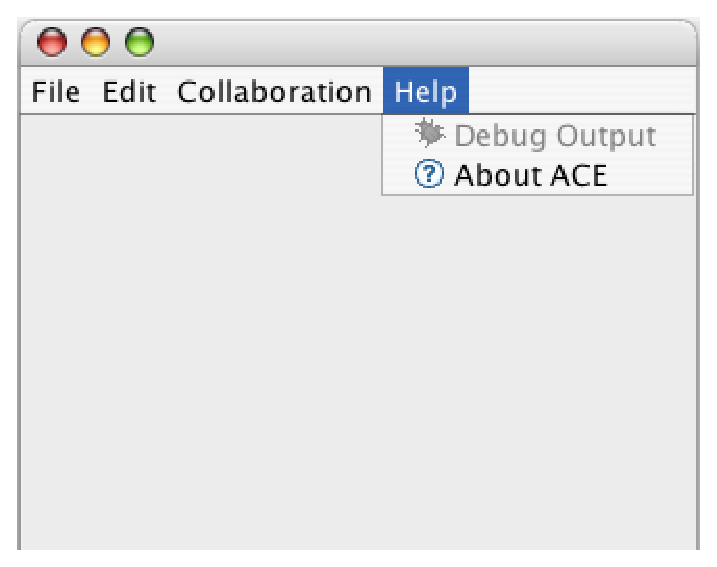
\includegraphics[height=1.78in, width=2.28in]{../images/usermanual/menu_help.eps}
\caption{About Menu}
\label{menu_about}
\end{center}
\end{figure}

\begin{figure}[H]
\begin{center}
  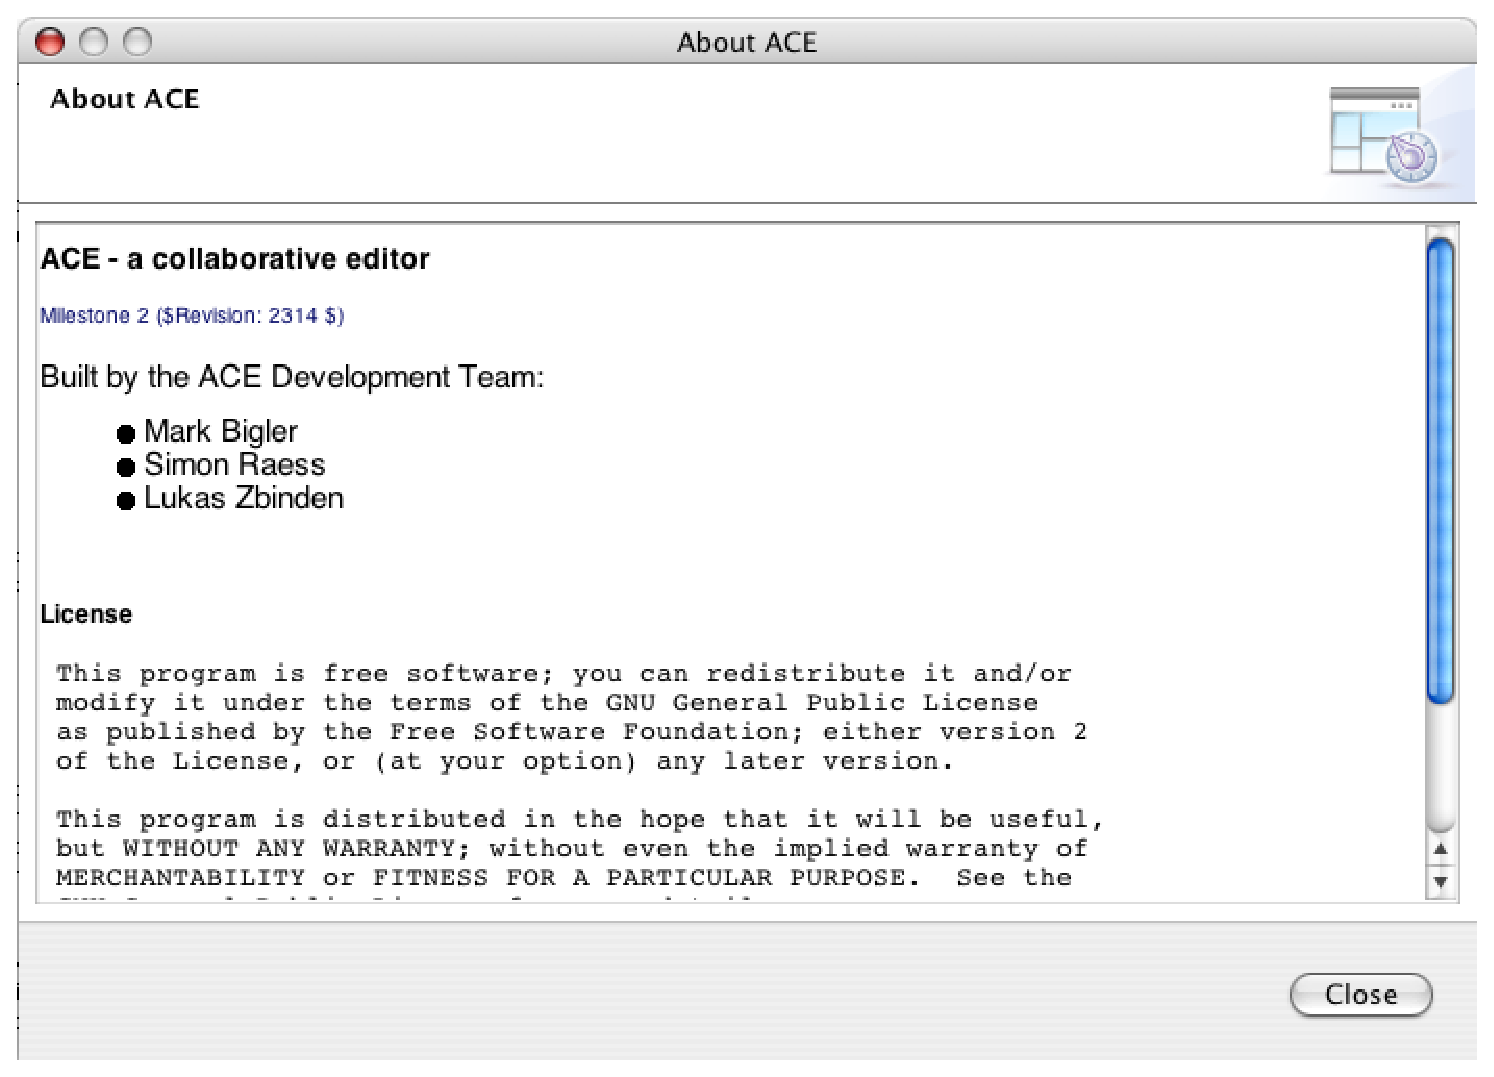
\includegraphics[height=3.48in, width=4.87in]{../images/usermanual/ace_about.eps}
\caption{About Dialog}
\label{dialog_about}
\end{center}
\end{figure}



\newpage
% 4. FIRST STEPS
\section{First Steps}
\label{first_steps}

% 4.1 CREATE
\subsection{Create a new Document}
First of all, you need to create a new document to start writing text. There are three different ways to create a new document:
\begin{itemize}
\item click on the \textit{new document} button in the \textbf{toolbar}
\item select the \textbf{menu item} named \textit{New} in the \textit{File} menu
\item enter the \textbf{shortcut} \textit{CTRL+N}.
\end{itemize}

Once you created a new document it appears in the \textit{Document View} in the upper left side of your editor.

% 4.2 OPEN
\subsection{Open an existing Document}
To open a existing document you have three posibilites:
\begin{itemize}
\item click on the \textit{open document} button in the \textbf{toolbar}
\item select the \textbf{menu} item \textit{Open} in the \textit{File} menu
\item enter the \textbf{shortcut} \textit{CTRL+O}.
\end{itemize}

% 4.3 SAVE
\subsection{Save open Documents}
To save an open document that has been changed you have three posibilites:
\begin{itemize}
\item click on the \textit{save document} button in the \textbf{toolbar}
\item select the \textbf{menu} item \textit{Save} in the \textit{File} menu
\item enter the \textbf{shortcut} \textit{CTRL+S}.
\end{itemize}

If you save a document the first time then a save dialog will be displayed where you can specify the name and location of the file to be saved.

% 4.4 QUIT
\subsection{Quit}
This dialog appears when you want to quit the application while you have unsaved documents. You can choose between four actions:
\begin{itemize}
\item \textit{Cancel}: Closes the dialog without doing anything. The application does not exit.
\item \textit{Save All}: Saves all listed documents. You will be asked for each document to enter a document name if the document has not been saved before.
\item \textit{Save None}: Saves none of the listed documents and quits the application.
\item \textit{Save Selected}: Saves only the selected files and quits the application. If a selected file has not been saved before you will be asked to enter a document name.
\end{itemize}

\begin{figure}[H]
\begin{center}
  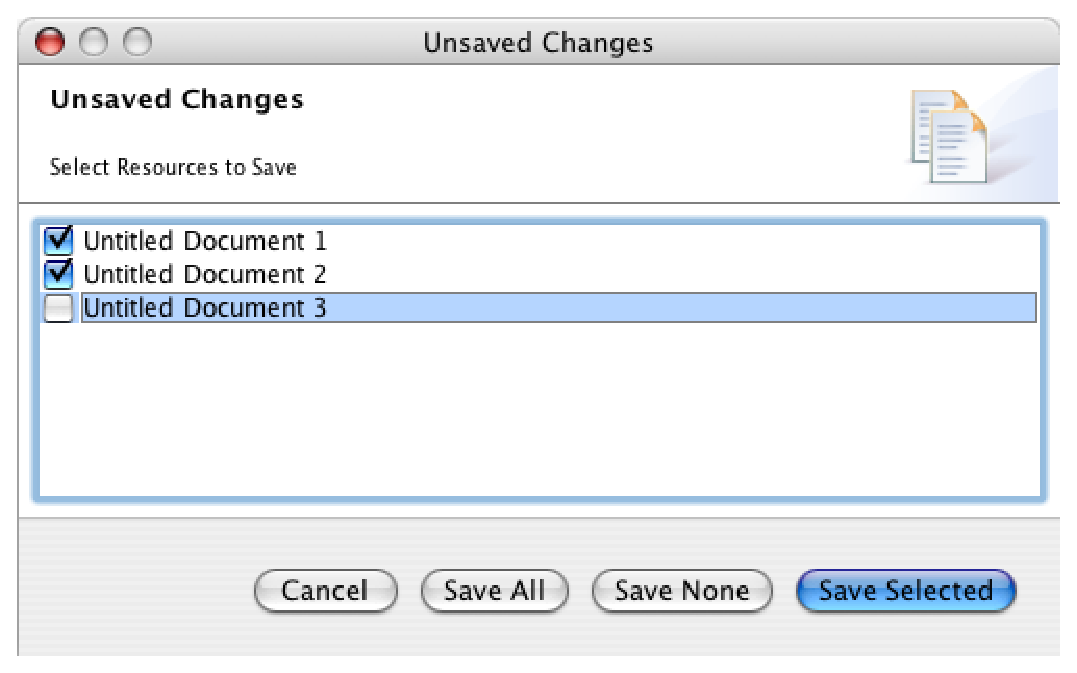
\includegraphics[height=3.20in, width=5.22in]{../images/usermanual/ace_savedialog.eps}
\caption{Save Dialog}
\label{dialog_quit_save}
\end{center}
\end{figure}




\newpage
% 5. NETWORKING
\section{Networking}
\label{sect_networking}

% 5.1 PUBLISH / CONCEAL
\subsection{Publish Documents}
\label{publish_conceal_documents}
Publishing documents is one of the features making ACE a collaborative editor. This is always the first step to edit documents with other users. To start collaborating, either you publish a document on your own and invite other users or you publish a document and other users request to join it themselves. \textbf{Note}: only published documents can be viewed by other users!

\begin{figure}[H]
\begin{center}
  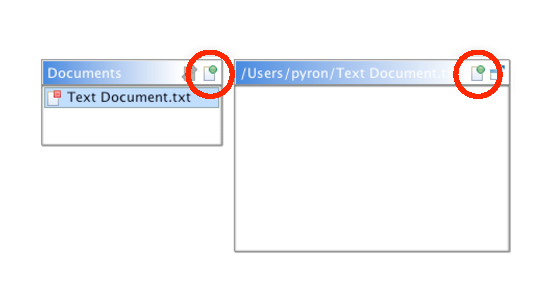
\includegraphics[height=1.32in, width=3.16in]{../images/usermanual/g_editor_view_publish.eps}
\caption{Publish Document}
\label{editor_view_publish}
\end{center}
\end{figure}

To publish a document you first need to select the document in the \textit{Document View}. After you have selected the document, you can click either the publish button at the top of the editor or the publish button at the top of the \textit{Document View}. Advanced users can use the shortcut \textit{CTRL+SHIFT+P}.

\begin{figure}[H]
\begin{center}
  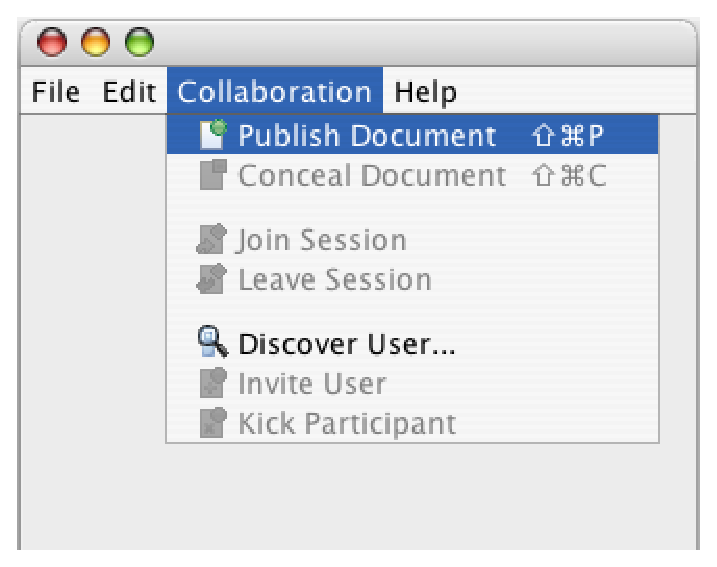
\includegraphics[height=1.78in, width=2.28in]{../images/usermanual/menu_collab_publish.eps}
\caption{Publish Document (Menu)}
\label{menu_publish}
\end{center}
\end{figure}

\subsection{Conceal Documents}
To conceal (unpublish) a document, select it and click on the conceal button (marked red in the figure \ref{editor_view_conceal}). After a document is concealed, all participants that have been writing in the document receive a notification that the session is over. ACE maintains a local copy of the document for each user.

\begin{figure}[H]
\begin{center}
  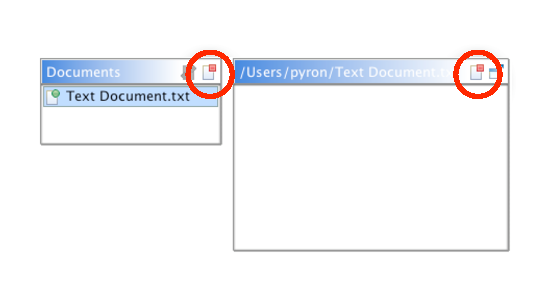
\includegraphics[height=1.32in, width=3.16in]{../images/usermanual/g_editor_view_conceal.eps}
\caption{Conceal Document}
\label{editor_view_conceal}
\end{center}
\end{figure}

You can use the action in the \textit{collaboration menu} to conceal the document. Advanced users can use the shortcut \textit{CTRL+SHIFT+C}.

\begin{figure}[H]
\begin{center}
  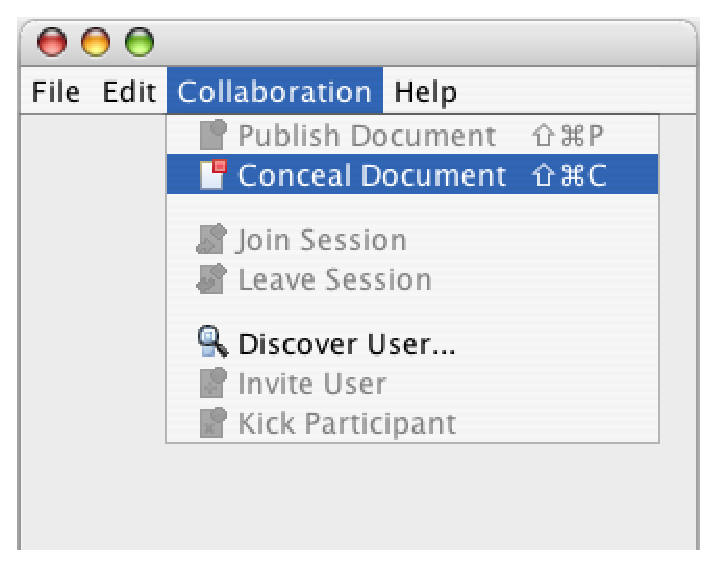
\includegraphics[height=1.78in, width=2.28in]{../images/usermanual/menu_collab_conceal.eps}
\caption{Conceal Document (Menu)}
\label{menu_conceal}
\end{center}
\end{figure}

% 5.2 INVITE / KICK
\subsection{Invite Users}
\label{invite_kick_users}
After you have published a document (see section \ref{publish_conceal_documents}) you can invite users. Select the document in the \textit{Document View} and then the user you want to invite from the \textit{User View}. Then you can either click the invite button in the view toolbar of the \textit{User View}

\begin{figure}[H]
\begin{center}
  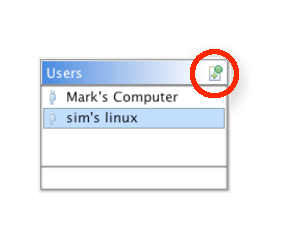
\includegraphics[height=2.64in, width=3.5in]{../images/usermanual/g_uview_invite.eps}
\caption{Invite User}
\label{g_uview_invite}
\end{center}
\end{figure}

or use the action from the \textit{collaboration menu}.

\begin{figure}[H]
\begin{center}
  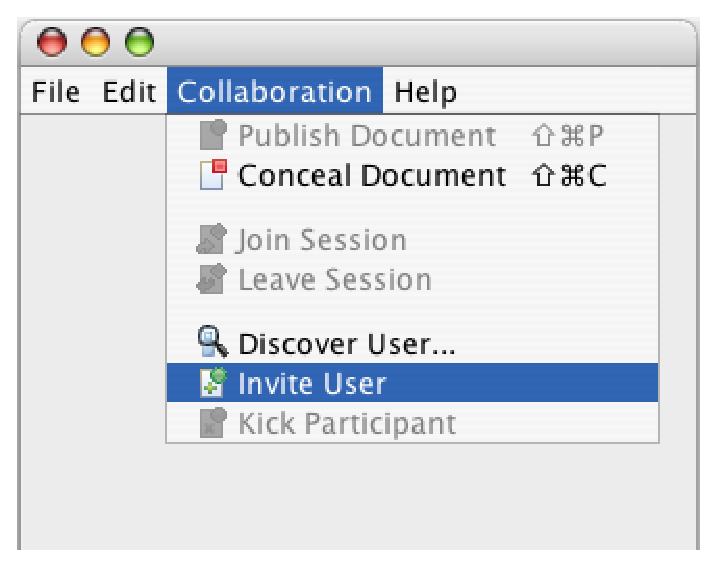
\includegraphics[height=1.78in, width=2.28in]{../images/usermanual/menu_collab_invite.eps}
\caption{Invite User (Menu)}
\label{menu_collab_invite}
\end{center}
\end{figure}

\subsection{Kick Users}
The inverse operation of inviting is kicking. This function has been added to \textit{remove} misbehaving participants from the session. Only the publisher of a document can kick users. 

\textbf{Note}: after you have kicked a participant, ACE automatically puts him on a blacklist, which makes it impossible for that user to rejoin the session (see section \ref{join_leave_documents} for more details about joining). To remove the user from the blacklist the publisher can reinvite the kicked user.

\begin{figure}[H]
\begin{center}
  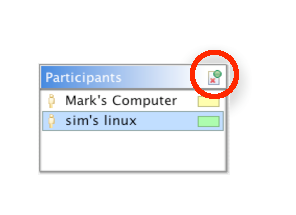
\includegraphics[height=2.42in, width=3.5in]{../images/usermanual/g_pview_kick.eps}
\caption{Kick User}
\label{g_pview_kick}
\end{center}
\end{figure}

To kick a user select the published document in the \textit{Document View}, the user you want to kick in the \textit{Participant View} and press the \textit{kick button} in the toolbar of the \textit{Participant View} or use the \textit{Kick Participant} entry from the \textit{Collaboration} menu.

\begin{figure}[H]
\begin{center}
  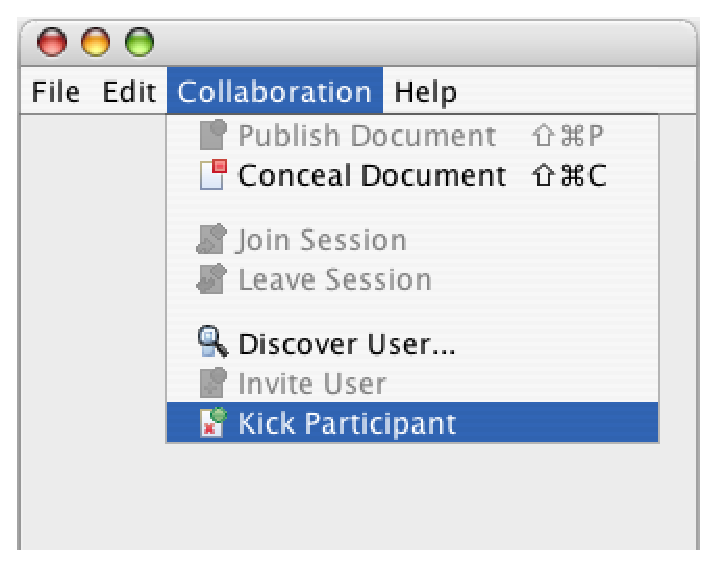
\includegraphics[height=1.78in, width=2.28in]{../images/usermanual/menu_collab_kick.eps}
\caption{Kick User (Menu)}
\label{menu_collab_kick}
\end{center}
\end{figure}

% 5.3 JOIN / LEAVE
\subsection{Join Network Documents}
\label{join_leave_documents}
To participate in other user's documents you need to join such a document. Basically you can join all the documents that are listed in the \textit{browse view}. Select the corresponding document and press the join button, click on the \textit{Join Session} in the \textit{Collaboration} menu or simple double click on it.

\begin{figure}[H]
\begin{center}
  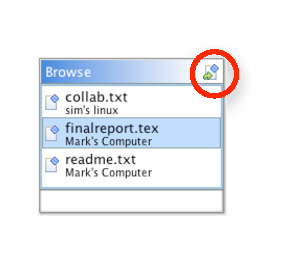
\includegraphics[height=2.94in, width=3.5in]{../images/usermanual/g_bview_join.eps}
\caption{Join Document}
\label{g_bview_join}
\end{center}
\end{figure}

\begin{figure}[H]
\begin{center}
  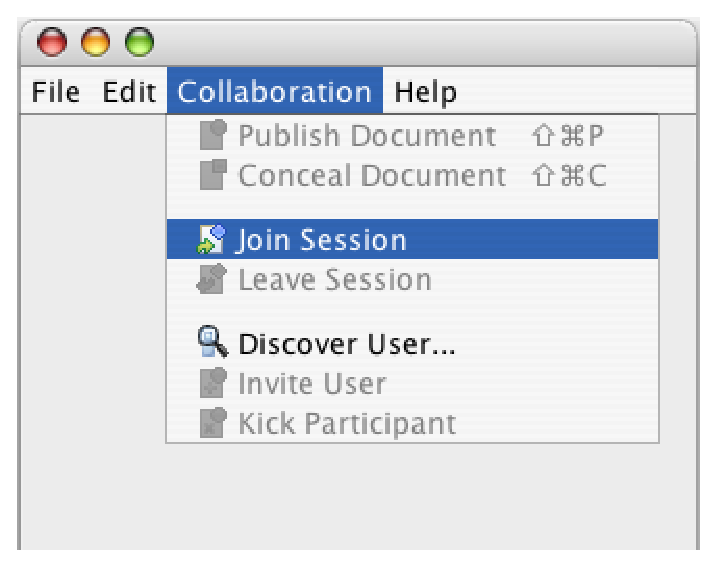
\includegraphics[height=1.78in, width=2.28in]{../images/usermanual/menu_collab_join.eps}
\caption{Join Document (Menu)}
\label{menu_collab_join}
\end{center}
\end{figure}

This sends a join request to the publisher of the document. The publisher (owner) receives a notification and he can either \textit{accept} or \textit{deny} your join request. If he accepts your join request you become a participant and you can start writing on your own in the joined document. See section \ref{collaborative_editing} for more details about collaborative editing.

\subsection{Leave Network Documents}
If you do not want to participate any longer in an editing session, you can leave. Select the document in the \textit{Document View} and press the leave button or use the menu item \textit{Leave Session} in the \textit{Collaboration}�menu. You can also close the document, in which case you also automatically leave the session.
\begin{figure}[H]
\begin{center}
  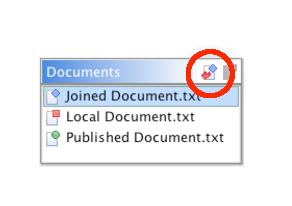
\includegraphics[height=2.3in, width=3.5in]{../images/usermanual/g_dview_leave.eps}
\caption{Leave Document}
\label{g_dview_leave}
\end{center}
\end{figure}

\begin{figure}[H]
\begin{center}
  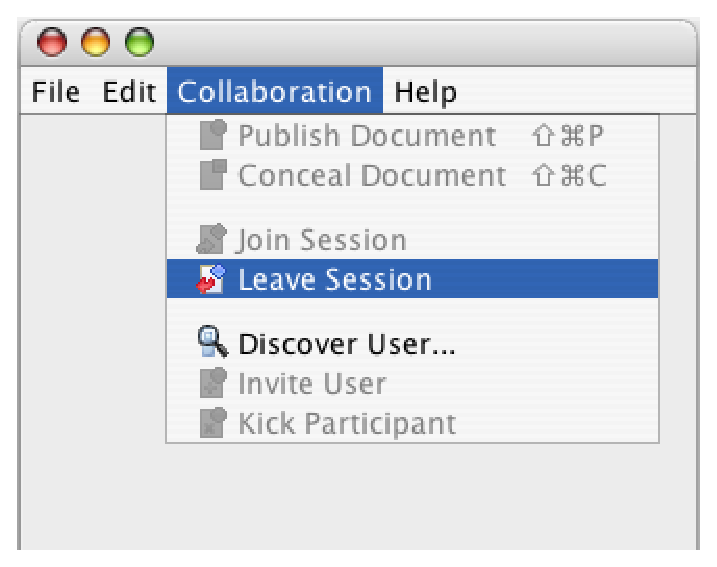
\includegraphics[height=1.78in, width=2.28in]{../images/usermanual/menu_collab_leave.eps}
\caption{Leave Document (Menu)}
\label{menu_collab_leave}
\end{center}
\end{figure}


% 5.4 DISCOVER
\subsection{Discover Users}
ACE automatically detects all other users on the same local area network. If you want to invite people from other networks (e.g. from another company or over the Internet) you must explicit discover them. Click in the \textit{Discover User} item in the \textit{Collaboration} menu. This will open the dialog shown in figure \ref{discover_dialog}.

\begin{figure}[H]
\begin{center}
  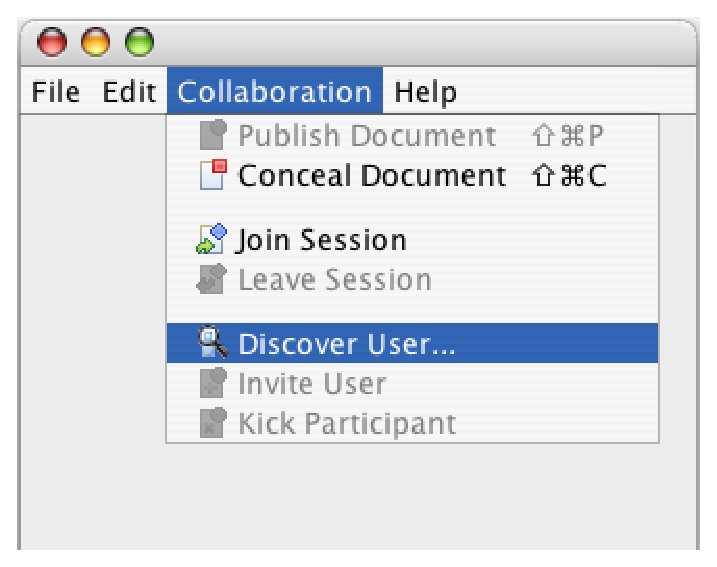
\includegraphics[height=1.78in, width=2.28in]{../images/usermanual/menu_collab_discover.eps}
\caption{Discover User Menu}
\end{center}
\end{figure}

Enter the IP address of the user you want to discover and press ok. Your own IP address is shown at the bottom of ACE all the time. The other user needs to give you his IP and you can discover him then.

\begin{figure}[H]
\begin{center}
  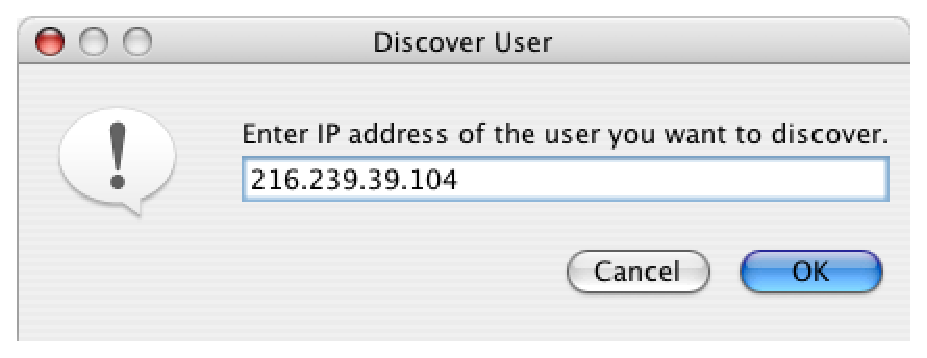
\includegraphics[height=1.08in, width=2.98in]{../images/usermanual/ace_discover.eps}
\caption{Discover User Dialog}
\label{discover_dialog}
\end{center}
\end{figure}

If you enter an invalid IP address the following dialog pops up:

\begin{figure}[H]
\begin{center}
  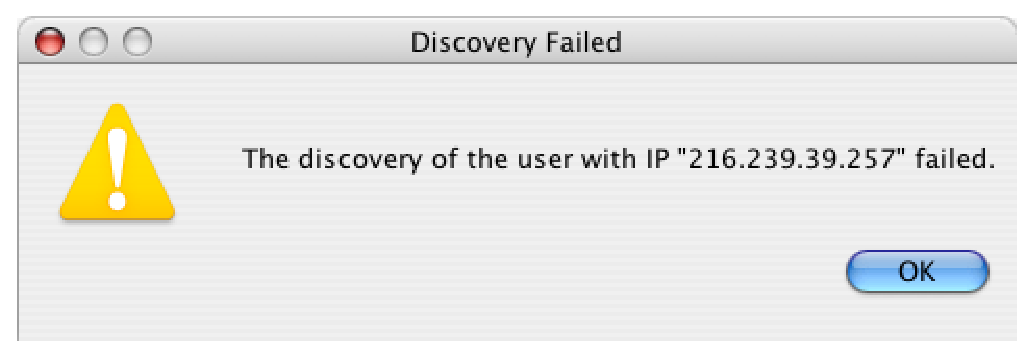
\includegraphics[height=1.08in, width=3.38in]{../images/usermanual/discover_failed_inv_ip.eps}
\caption{Discover Failed Dialog}
\end{center}
\end{figure}

When the IP you entered was valid but the contacted computer has no instance of ACE running then you receive the following error message:

\begin{figure}[H]
\begin{center}
  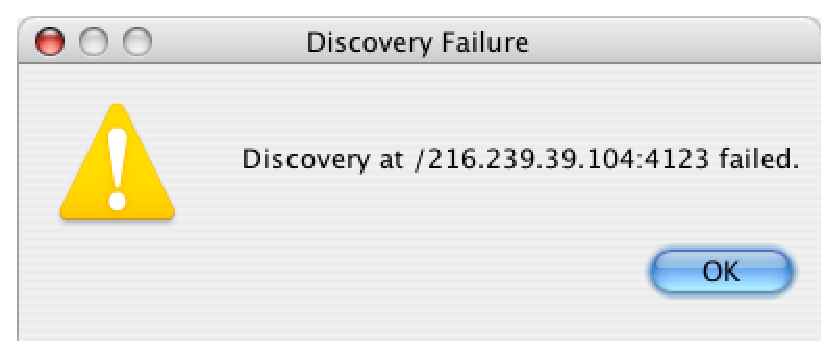
\includegraphics[height= 1.08in, width=2.68in]{../images/usermanual/discover_failed_no_ace.eps}
\caption{Discover Failed Dialog}
\end{center}
\end{figure}

If the discovery was successful the discovered user is added to the \textit{User View}. It cannot be distinguished from an automatically discovered user.

\newpage
% COLLAB_EDITING
\subsection{Collaborative Editing}
\label{collaborative_editing}
For each published document there is a participant list. Select the document and the \textit{Participant View} will show you the actual list of users participating in this document editing session. Each user (participant) has his own color which is used to highlight the text he wrote:

\begin{figure}[H]
\begin{center}
  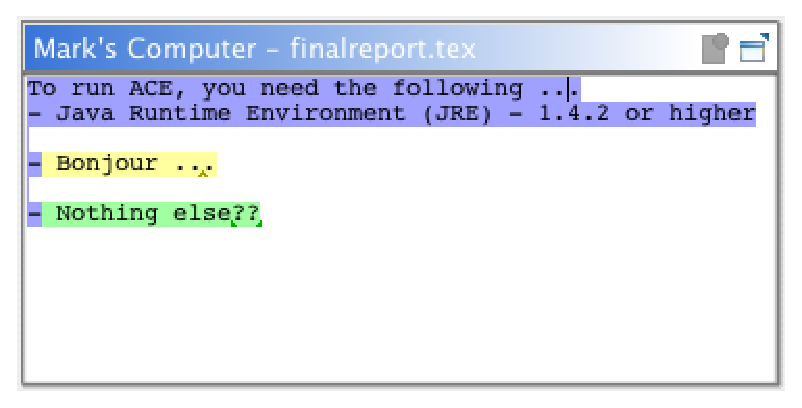
\includegraphics[height=1.25in, width=2.56in]{../images/usermanual/editor_collab_3users.eps}
\caption{Three users in the same document}
\end{center}
\end{figure}

After a participant left (either he explicitly left or he was kicked by the owner), his text will be highlighted in gray color. In case he joins the document again the grayed-out text he wrote will be colored again in his former color.

\begin{figure}[H]
\begin{center}
  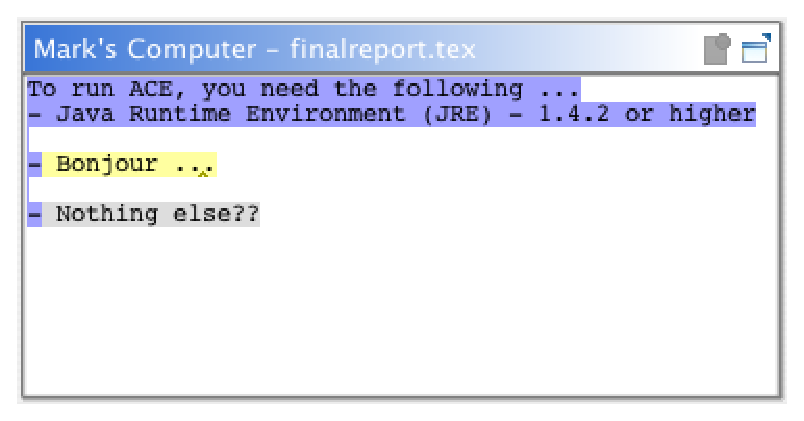
\includegraphics[height=1.29in, width=2.57in]{../images/usermanual/editor_collab_user_left.eps}
\caption{After one user left the document}
\end{center}
\end{figure}


\newpage
\listoffigures

\end{document}
